\documentclass{article}
\usepackage[normalem]{ulem}
\usepackage[14pt]{extsizes}
\usepackage[utf8]{inputenc}
\usepackage[T2A]{fontenc}
\usepackage{amsmath}
\usepackage{amssymb}
\usepackage{mathtools}
\usepackage{hyperref}
\usepackage{amsfonts}
\usepackage{cmap}
\usepackage{multicol}
\usepackage{comment}
\usepackage[parfill]{parskip}

\usepackage{listings}
\usepackage{color}
\usepackage{colortbl}
\usepackage{xcolor}
\usepackage[left=1.5cm,right=2cm,top=2cm,bottom=2cm,bindingoffset=0.1cm]{geometry}
\usepackage[russian]{babel}
\usepackage[pdf]{graphviz}
\usepackage{tikz}
\usepackage{pgfplots}
\usepgfplotslibrary{polar}
\usepackage{etoolbox} % <--- added
\AtBeginEnvironment{enumerate}{\linespread{.84}\selectfont}
\newcommand{\ctd}{\begin{flushright} $\square$ \end{flushright}}
%%% Работа с картинками
\usepackage{graphicx}  % Для вставки рисунков
  % папки с картинками
\setlength\fboxsep{3pt} % Отступ рамки \fbox{} от рисунка
\setlength\fboxrule{1pt} % Толщина линий рамки \fbox{}
\pagenumbering{gobble}



\hypersetup{
    colorlinks=true,
    linkcolor=blue,
    filecolor=magenta,      
    urlcolor=blue,
    pdftitle={Alfo},
    pdfpagemode=FullScreen,
    }
\lstset{ %
  language=C++, % the language of the code
  basicstyle=\footnotesize\ttfamily, % the size of the fonts that are used for the code
  numbers=left, % where to put the line-numbers
  numberstyle=\footnotesize\color{black},  % the style that is used for the line-numbers
  stepnumber=0, % the step between two line-numbers. If it's 1, each line 
       % will be numbered
  numbersep=0.7em,       % how far the line-numbers are from the code
  backgroundcolor=\color{white!95!gray}, % choose the background color. You must add \usepackage{color}
  showspaces=false,      % show spaces adding particular underscores
  showstringspaces=false,% underline spaces within strings
  showtabs=false,        % show tabs within strings adding particular underscores
  frame=single, % adds a frame around the code
  rulecolor=\color{black},        % if not set, the frame-color may be changed on line-breaks within not-black text (e.g. commens (green here))
  tabsize=2,    % sets default tabsize to 2 spaces
  %captionpos=b,% sets the caption-position to bottom
  breaklines=true,       % sets automatic line breaking
  breakatwhitespace=false,        % sets if automatic breaks should only happen at whitespace
  %title=\lstname,       % show the filename of files included with \lstinputlisting;
       % also try caption instead of title
  identifierstyle=\color{black!50!green},  
  keywordstyle=\color{blue},      % keyword style
  commentstyle=\color{gray},      % comment style
  stringstyle=\color{purple},      % string literal style
  escapeinside={\%*}{*)},% if you want to add a comment within your code
  morekeywords={n,k},    % if you want to add more keywords to the set
  morecomment=[l][\color{black!50!green}]{\#}, % to color #include<cstdio> 
  morecomment=[s][\color{gray!50!black}]{/**}{*/}
}

\usepackage{amsmath,amssymb}
\usepackage{ stmaryrd }
\usepackage{ dsfont }
\usepackage{ tipa }
\usepackage{amsthm}

\newcommand{\updownarrows}{\mathbin\uparrow\hspace{-.5em}\downarrow}
\newcommand{\downuparrows}{\mathbin\downarrow\hspace{-.5em}\uparrow}
\newcommand{\defeq}{\stackrel{\mathclap{\normalfont\mbox{def}}}{=}}
\newcommand{\defLeftrightarrow}{\xLeftrightarrow{def}}


\usepackage{fancyhdr}
\pagestyle{fancy}
\fancyhf{}

\fancyhead[C]{Алгоритмы и структуры данных} % Центральный заголовок
\fancyhead[L]{КТ ИТМО - 1 Семестр}
\fancyhead[R]{Первеев Михаил}


\usepackage{tocloft}

\renewcommand{\cftsecfont}{\normalfont}
\renewcommand{\cftsecpagefont}{\normalfont}
\renewcommand{\cftsubsecfont}{\normalfont}
\renewcommand{\cftsubsecpagefont}{\normalfont}


\setlength{\cftsecindent}{0em}
\setlength{\cftsubsecindent}{0em}
\cftsetpnumwidth{0em}
\cftsetrmarg{0em}

\newcommand{\deff}[1]{\underline{\textbf{#1}}}
\newcommand{\thmm}[1]{\underline{\textbf{#1}}}
\newcommand{\prooff}[1]{\textbf{\underline{Доказательство:}} \\ }
\newcommand*\xor{\mathbin{\oplus}}

\title{Алгоритмы и структуры данных.}
\author{Чепелин В.А.}
\date{}

\begin{document}
\maketitle


\tableofcontents
\pagebreak

\section{ О-нотация.}

\begin{lstlisting}[mathescape]
    int m = INT_MAX;
    for (int i = 0; i < n; i++) {
        if (a[i] < m) {
            m = a[i];
        }
    }
\end{lstlisting}
Хотим понять за сколько работает алгоритм. Но измерять в секундах/миллисекундах и т.п довольно странно (процессоры разные и т.п).

Тогда люди придумали \deff{RAM-модуль}. Мы умеем за 1 операцию:

\begin{enumerate}
    \item  Обратиться к памяти и получить что-то.
    \item Записать в память что-то.
    \item Делать операции с числами.
\end{enumerate}

Тогда посчитаем T(n) для этой операции: $T(n) = 1 + (1+n+3n)+2n=8n+2$

Ну такая запись нам почти ничего не дает. Введем некоторые определения:

$f(n)=O(g(n))$, если $\exists N,c>0: \forall n>N: f(n) \leq c g(n)$

O(n) --- \deff{ограничивает сверху}.

$f(n) = \Omega (g(n))$, если $\exists N,c>0: \forall n>N: f(n) \geq c g(n)$

$\Omega(n)$ --- \deff{ограничивает снизу}.
.
$f(n)=\theta(g(n))$, если$\exists N,c_1,c_2>0: \forall n>N: c_2 g(n)\leq f(n) \leq c_1 g(1)$

$\theta(n)$ --- \deff {ограничивает и сверху и снизу}.

Теперь будем каждую T(n) оценивать O(g(n)) и измерять кол-во операций так.
Тогда T(n) = 8n+2 = O(n)

Заметим, что любые константы или многочлены внутри  O, можно убирать/упрощать.

O(2n)=O(n) или O($n^2$-n)=O($n^2$).
Разберем еще пример:

\begin{lstlisting}[mathescape]
for (int i = 0; i < n; i++) {
        for (int j = i; j < n; j++) {
            if (a[j] > a[j + 1]) {
                swap(a[j], a[j + 1])
            }
        }
    }
\end{lstlisting}
Ну $T(n) = 1+2+\dots+n=\tfrac{n(n+1)}{2}=O(n^2)$

И теперь понятно как считать for,while и тому подобное. Но что нам делать с рекурсивными формулами? Например такой:
\begin{lstlisting}[mathescape]
int f(int n) {
    if (n == 0) return 0;
    else return 1 + f(n - 1);
}
\end{lstlisting}

Запишем наше время тоже в рекурсивном виде: T(n) = 1 + T(n-1). И тут можно посмотреть, что будет ровно n операций. Или вот такой:

\begin{lstlisting}[mathescape]
int f(int n) {
    if (n == 0) return 0;
    else return 1 + f(n / 2);
}
\end{lstlisting}
Напишем наше время тоже в рекурсивном виде: T(n) = 1 + T(n/2). 
И если немножко подумать, то T(n) = O(logn) (причем необязательно указывать у логарифма основание).

Но что делать когда у нас допустим $T(n)=2T(\frac{n}{2})+n$. Тут уже не очев очевидно, но можно предположить, что здесь O(nlogn). Как нам это доказать?

По индукции! База: для n равному 5 верно, докажем для более больших!

Пусть верно для всех $k<n$, докажем для n.

$T(n) = 2T(\frac{n}{2})+n=2\frac{n}{2}\log\frac{n}{2} =n(\log n-1)<n\log n$.Верно

Иногда надо подгонять функцию. То есть например вместо nlogn подставлять nlogn - $\frac{n}{2}$

\deff{Мастер теорема.}

$T(n)=a*T(\frac{n}{b}) + n^c$.

Тогда при $T(1)=const$:

1) $c<\log_{b}a \Rightarrow T(n) = O(n^{\log_ba})$

2) $c=\log_{b}a \Rightarrow T(n) = O(n^c\log n)$

3) $c>\log_{b}a \Rightarrow T(n) = O(n^c)$

\prooff{} Представим в виде дерева ветвления. На первом слое 1 вершина с кол-вой операций $n^c$, на втором a вершин с $(\frac{n}{b})^c$ операций и так далее.

 Тогда наше кол-во операций будет таквым:
 
 $\sum\limits_{i=0}^{\log_bn}a^i*(\cfrac{n}{b^i})^c =n^c \sum\limits_{i=0}^{\log_bn} (\cfrac{a}{b^c})^i  $

 И есть 3 случая:

 1) $(\frac{a}{b^c})^i=1$, тогда $\sum\limits_{i=0}^{\log_bn} (\frac{a}{b^c})^i =n^c\log_bn$ чтд.

 2) $(\frac{a}{b^c})^i>1$, тогда $\sum\limits_{i=0}^{\log_bn} (\frac{a}{b^c})^i =n^c * \frac{q^{\log_bn+1}-1}{q-1}<n^c *q^{\log_bn} = n^c (\frac{a}{b^c})^{\log_bn} =n^{\log_ba}$ чтд.

 3) $(\frac{a}{b^c})^i<1$, тогда геом прогрессия убывающая ч.т.д

 (нужные нам неравенства выходят преобразованием этих в вид логарифмов)
 \pagebreak
 \section{Теория вероятности.}

 \deff{Вероятностное пространство} --- $\Omega $ - мн-во элементарных исходов (конечное или счетное). p: $\Omega \rightarrow [0,1]$, такая что
 $\sum\limits_{w \in \Omega}p(w) = 1$.

 \textbf{Примеры:}

\begin{enumerate}
    

 \item  Кидаем честную монетку. $\Omega = {O,R}, p(O)=\frac{1}{2}, p(R)=\frac{1}{2}$.

 \item Кидаем нечестную монетку. $\Omega = {O,R}, p(O)=p, p(R)=1-p$.

 \item Игральный кубик. $\Omega = {1,2,3,4,5,6}, p(i)=\frac{1}{6}$.

 \item Бесконечная монетка. $\Omega = \mathbb{N} =\{w_1,w_2,\ldots,w_i,\ldots\}$.

 $p(w_i)=(\frac{1}{2})^i$.
 \end{enumerate}

\deff{Произведение вероятностное пространство} --- Пусть есть 2 вероятностных пространств: $\Omega_1, p_1$ и $\Omega_2, p_2$. Тогда их произведение это такое вероятностное пространство, что $\Omega = \Omega_1 \times \Omega_2$, а $p(\langle w_1,w_2 \rangle) = p_1(w_1) * p_2(w_2)$.

\deff{Событие} --- любое подмножество множества  элементарных исходов. При чем вероятность этого события считается, как сумма всех вероятностей.

С событиями можно сделать то же самое, что и с множествами.

\deff{Независимые события} --- A, B - независимы, если $p(A \wedge B) = p(A) P(B)$.

\deff{Случайная величина} --- функция $X: \Omega \rightarrow R$.

\deff{Плотность случайной величины} --- функция, которая по значению случ. величины, говорит вероятность, с которой она могла выпасть. $f_X(t) = P(X=T)$

\textbf{Пример.} $D_6$ - пространство игрального кубика.

Рассмотрим $D_6^2$

$X(w_1,w_2)=w_1+w_2$. Значения случайной величины в таком случае [2,12]. 

$f_X(2) = \frac{1}{36}, f_X(3)=\frac{1}{18}, \ldots, f_X(12)=\frac{1}{36}$, Можно рисовать графики.

\deff{Математическое ожидание случайной величины } --- $E(X)$- мат. ожидание величины $X$. По определению:

$E(X) = \sum\limits_{w \in \Omega} X(w)p(w)$.

\textbf{Пример.} Мат. ожидание для кубика $=1\cdot \frac{1}{6}+\ldots +6\cdot \frac{1}{6} = 3,5$.

\thmm{Теорема.} Пусть есть 2 случайные величины $X,yY$ и $\lambda \in \mathbb{R}$. Тогда:
\begin{enumerate}
    \item[1)] $E(\lambda X) = \lambda E(X)$
    \item[2)] $E(X+Y)=E(X)+E(Y)$
\end{enumerate}
Доказательство тривиально через определение.
\pagebreak
\section{Cортировки.}
\subsection*{Квадратичные сортировки.}
\begin{enumerate}
    \item \textbf{Пузырьком} (похоже на пузырек, который всплывает со дна):
    \begin{lstlisting}[mathescape]
   for (int i = 0; i < n; i++) {
    for (int j = 0; j < i; j++) {
      if (digitals[j] > digitals[j + 1]) {
         swap(a[j],a[j+1]);
      }
    }
  }
\end{lstlisting}
    \item \textbf{Вставками} - на i-ом ходу отсорчен префикс длины i:
    \begin{lstlisting}[mathescape]
    for(int i = 1;i < n;i++)     
	   for(int j = i;j > 0 && x[j-1] > x[j]; j--) 
			swap(x[j-1],x[j]);        
     \end{lstlisting}
    \item \textbf{Выбором}:
    \begin{lstlisting}
     int min, temp; 
    for (int i = 0; i < size - 1; i++){
        min = i;
        for (int j = i + 1; j < size; j++){
            if (num[j] < num[min])
                min = j;      
        }
        if (min == i) continue;  
        temp = num[i];      
        num[i] = num[min];
        num[min] = temp;
    }
    \end{lstlisting}
\end{enumerate}
\subsection*{QuickSort или Сортировка Хоара.}

\deff{Быстрая сортировка (quick sort)} — один из самых известных и широко используемых алгоритмов сортировки. Среднее время работы $O(n \log n)$. Хотя время работы алгоритма для массива из n элементов в худшем случае может составить O($n^2$).

Быстрый метод сортировки функционирует по принципу \uline{разделяй и властвуй}:

Массив a[l…r] разбивается на два подмассива a[l…q] и a[q+1…r], таких, что каждый элемент a[l…q] меньше или равен a[q], который в свою очередь, не превышает любой элемент подмассива a[q+1…r]. Индекс вычисляется в ходе процедуры разбиения.

Подмассивы a[l…q] и a[q+1…r] сортируются с помощью рекурсивного вызова процедуры быстрой сортировки.

Вот код:
\begin{lstlisting}[mathescape]
#include <bits/stdc++.h>
using namespace std;

vector<int> a;

// [left, right]
int partition(int left, int right) {
    int v = a[(left + right) / 2];
    int i = left, j = right;
    
    while (i <= j) { 
        while (a[i] < v)
            i++;
        while (a[j] > v)
            j--;
        if (i >= j) 
           break;
        swap(a[i++], a[j--]);
    }
    
    return j;
}

// [left, right]
void my_sort(int left, int right) {
    if (left < right) {
        int q = partition(left, right);
        my_sort(left, q);
        my_sort(q + 1, right);
    }
}

int main() {
    int n;
    cin >> n;
    
    a.resize(n);
    for (auto &i : a) cin >> i;
    
    my_sort(0, n - 1);
    for (auto &i : a) cout << i << ' ';
}
 \end{lstlisting}

Объясним асимптотику:

Посчитаем тогда чему равно мат. ожидание $E(T(n))$ нашего алгоритма. 

$E(T(n)) = n + \frac{1}{n}\sum\limits_{i=0}^{n-1}(E(T(i)) + E(T(n-i+1)))$ 

$n E(T(n)) = n^2 + 2 \sum\limits_{i=0}^{n-1} E(T(i))$

Подставим n-1 и вычтем:

$nE(T(n))=(n+1) T(n-1) +2n$ --- тут я нагло оцениваю сверху. 

Поделим на $n(n-1).$

$\displaystyle \frac{E(T(n))}{n+1}=\frac{E(T(n-1))}{n}+\frac{2}{n+1}$ ---  работает для любого n так что подставлю вместо  $\displaystyle \frac{E(T(n-1))}{n}$ его значение. Буду делать так, пока T не равно 1:

$E(T(n)) = 2(n+1)(\frac{1}{1}+\frac{1}{2}+\ldots + \frac{1}{n+1})$

$T(n) = O(n\log n)$

\subsection*{MergeSort.}

\deff{Merge sort} - сортировка слиянием O(n logn)

Алгоритм использует принцип \uline{разделяй и властвуй}: задача разбивается на подзадачи меньшего размера, которые решаются по отдельности, после чего их решения комбинируются для получения решения исходной задачи. Конкретно процедуру сортировки слиянием можно описать следующим образом:

Если в рассматриваемом массиве один элемент, то он уже отсортирован ---алгоритм завершает работу.
Иначе массив разбивается на две части, которые сортируются рекурсивно.
После сортировки двух частей массива к ним применяется процедура слияния, которая по двум отсортированным частям получает исходный отсортированный массив.

Слияние:
Эта процедура заключается в том, что мы сравниваем элементы массивов (начиная с начала) и меньший из них записываем в финальный. И затем, в массиве у которого оказался меньший элемент, переходим к следующему элементу и сравниваем теперь его. В конце, если один из массивов закончился, мы просто дописываем в финальный другой массив. После мы наш финальный массив записываем вместо двух исходных и получаем отсортированный участок.
Код:

\begin{lstlisting}[mathescape]
#include <bits/stdc++.h>
using namespace std;

vector<int> a;

// [left, right)
vector<int> my_merge(int left, int mid, int right) {
    vector<int> res;
    int p1 = left, p2 = mid;
    
    while (p1 < mid && p2 < right) {
        if (a[p1] < a[p2]) res.push_back(a[p1++]);
        else res.push_back(a[p2++]);
    }
    
    while (p1 < mid)   res.push_back(a[p1++]);
    while (p2 < right) res.push_back(a[p2++]);
    
    return res;
}

// [left, right)
void my_sort(int left, int right) {
    if (right - left <= 1) return;
    
    int mid = (left + right) / 2;
    my_sort(left, mid);
    my_sort(mid, right);
    
    vector<int> vec = my_merge(left, mid, right);
    for (int i = 0; i < (right - left); i++)
        a[left + i] = vec[i];
}

int main() {
    int n;
    cin >> n;
    
    a.resize(n);
    for (auto &i : a) cin >> i;
    
    my_sort(0, n);
    for (auto &i : a) cout << i << ' ';
}

\end{lstlisting}

\subsection *{Почему нельзя быстрее n log n?}

Единственная доступная операция --- сравнить 2 элемента. Докажем, что тогда нельзя сортить быстрее.

(для простоты объяснения все элементы попарно различны)

У каждого сравнения 2 результата.  Построим дерево всех возможных сравнений. Пришли в какой-то лист = выполнили последовательность сравнений, получили итоговое состояние. Таких листов должно быть $n!$(так как разные перестановки не могут давать одну перестановку). Таких $2^h$, где h - глубина дерева. Заметим, что  h >=$log(n!)$, что $h>\Omega(n\log n)$. Откуда быстрее $n\log n $ нельзя.

\subsection *{Сортировка подсчетом.}

 Она работает за O(n), но с очень большой константой. Это алгоритм сортировки, в котором используется диапазон чисел сортируемого массива для подсчёта совпадающих элементов. Применение сортировки подсчётом целесообразно лишь тогда, когда сортируемые числа имеют (или их можно отобразить в) диапазон возможных значений, который достаточно мал по сравнению с сортируемым множеством, например, миллион натуральных чисел меньших 1000.
 
Код:
\begin{lstlisting}[mathescape]
void countingSort(vector<int>& arr) {
      int max = max_element(arr.begin(), arr.end());
 	vector<int> count(max + 1, 0);

 	for (int elem : arr)
 		++count[elem];
	
 	int b = 0;
 	for (size_t i = 0; i <= max; i++) {
 		for (int j = 0; j < count[i]; j++) {
 			arr[b++] = i;
 		}
 	}	
 }
 \end{lstlisting}

 Пусть все числа массива $[0,k)$, чисел n, тогда сортировка подсчетом, просто создает массив длины k и идет по искомому массиву с числами. Пусть встретилось число a, тогда в массиве размера k по индексу a мы увеличиваем значение на 1. Потом просто проходимся по массиву длины k и для индекса i выводим столько чисел i, сколько было записано в массиве.

\pagebreak

 \section{k-ая порядковая статистика.}

$a_0,a_1,\ldots,a_n$. $k \in [0,n-1]$. Нужно найти k-ый элемент после сортировки. Отсюда следует очевидное решение за O(n log n). Хотим быстрее.

Вспомним quick sort. Мы научились разделять массив за O(n) на 2 части, где одна $\leq$ x, а другая $>$ x. Пусть в первую попало s. Если $k\leq s$ идем в левую, иначе идем в правую и ищем $k-s$ порядковую в правой части.  Оценим:

$T(n)=n + \cfrac{1}{n} (T(1)+\ldots T(n-1))$ --- оцениваем так же, как и в quick sort, но, в отличие от него, мы запускаемся только из одной половины.

$nT(n)=n^2 +(T(1)+\ldots T(n-1)$

$(n-1)T((n-1))=(n-1)^2 +(T(1)+\ldots T(n-2))$

Вычтем:

$nT(n) = 2n-1 + n T(n-1)$

И очевидно, что $T(n)=O(n)$.

Собрались как-то 5 мужиков, сели в баре и придумали алгоритм$\ldots$

\deff{Блум, Флойд, Пратт, Ривест, Тарьян или алгоритм пяти мужиков}. На практике его никто не использует.

Все n элементов входного массива разбиваются на группы по пять элементов, в последней группе будет n mod 5 элементов.

Сначала сортируется каждая группа, затем из каждой группы выбирается медиана.
Путем рекурсивного вызова поиска k-ой порядковой определяем медиану x
 из множества медиан (верхняя медиана в случае чётного количества).


 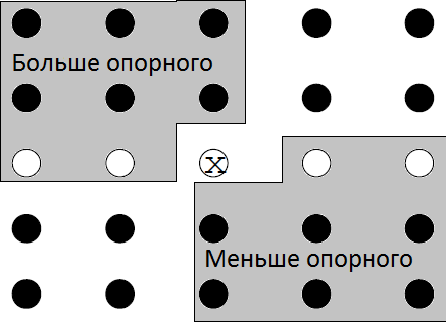
\includegraphics[width=9cm, height=6cm]{4.1.png}

 В данном примере в исходном массиве было 25 чисел. Разбили по  5 элементов. Нашли медиану( для лучшего понимания был отсорчен массив так, что центральная строчка отсорчена по убыванию (невозрастанию).)
 
 После каждого шага, мы знаем, что в точности $\cfrac{3n}{10}$, строго больше опорного, а  $\cfrac{3n}{10}$ меньше опорного.(это очевидно из обычных неравенств, на рисунке данные части были обведены и закрашены).

 Про остальные элементы(не закр. на рисунке) мы ничего не знаем. Заметим, что мы можем понять, где у нас лежит k-ая порядковая(либо в больше опорного и в клетках, про которые мы не знаем или в меньше опорного и в клетках, про которые мы ничего не знаем). Тогда запустимся рекурсивно от той части, в которой лежит наша k-ая порядковая. Тогда время работы будет:

$T(n) = T(\cfrac{n}{5}) + T(\cfrac{7n}{10}) +cn $, где c - какая-то константа.

 Ну и по индукции можно доказать, что T(n) = 10cn -- подходит в качестве оценки на время работы. Тогда асимптотика O(n).



\pagebreak
 \section{Кучи.}
 Что умеют? На английском heap.
 \begin{enumerate}
     \item getMin() --- доставать минимум
     \item add() --- добавлять в кучу
     \item extractMin() --- убирать из кучи минимум
 \end{enumerate}
 Мы будем говорить про \deff{Двоичную кучу.}
 
 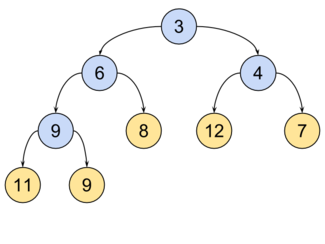
\includegraphics[width=10cm, height=6cm]{5.1.png}

 Вот так она выглядит. Ее суть в том, что  в каждой вершине мы храним число меньше либо равное ее детей. Как мы это храним? Можно создать отдельную структуру, которая хранит ссылку. Но мы каждую вершину будем хранить в массиве. Давайте корню присвоим нулевый индекс и так далее(как показано на рисунке)
 
  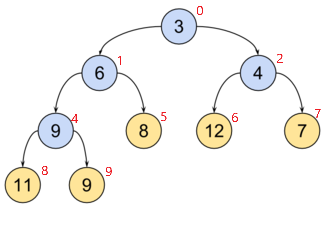
\includegraphics[width=10cm, height=6cm]{5.2.png}


Если мы увидем, то если есть вершина $i$, то у ее детей индексы $2i+1$,$2i+2$. Еще мы можем получить родителя $\frac{i-1}{2}$ и округлить вниз. Заметим, что у нас поддерживается инвариант $a[i]\leq min(a[2i],a[2i+1])$

\textbf{Как добавлять новый элемент?} Берем вершину и добавляем на самый нижний слой(если он занят, то создаем новый). Для примера мы хотим добавить вершину с числом 3.  Добавим.

 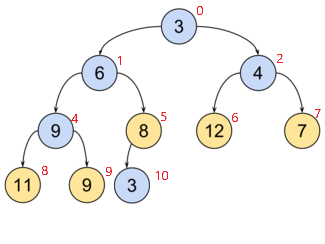
\includegraphics[width=10cm, height=6cm]{5.3.png}

Заметим, что у нас сломался инвариант: теперь значение в родителях не строго больше значения в ячейках. Чтобы это пофиксить, мы должны свапнуть значения с родителем несколько раз(Максимум log n swapов).(Я думаю, что каждому читателю очевидно то, почему это работает, так что пропустим). Называется это sift up.

\textbf{Как удалять минимум?}

Мы умеем на халяву удалять самый правый элемент самого нижнего уровня. Свапнем его с минимумом. Но инвариант у кучи сломался. Будем свапать его с минимальным ребенком и заметим, что ничего не ломается. Сделаем так несколько раз и все будет хорошо(Максимум log n swapoв)! Называется sift down.

\textbf{Как доставать минимум?}

Минимум лежит в ячейке с индексом 0, так что просто выводим его.

\textbf{Давайте добавим операцию decreaseKey().}

Че она умеет? По номеру вершины  уменьшать на сколько-то. Как мы это делаем? Берем вершину, понижаем и свапаем с верхней если что-то сломанно (Максимум log n swapoв). 

\textbf{Строить можно за O(n)}

Есть массив a. Хотим пошаманить с массивом, чтобы он представлял из себя кучу (без доп. памяти). Давайте каждым ходом будем добавлять в рассмотрение 1 элемент и чтобы подотрезок от 0 до k-1 был кучей (где k-номер хода).

Докажем по индукции, что мы так можем. База очевидна. Докажем для k, что это верно. Добавляем элемент в нашу кучу и делаем sift up. Работает за $n\log n$. 

Хотим за n. Давайте то же самое, но с конца. С конца у нас будут образовываться какие-то корректные кучи. Добавляем элемент и вызываем sift down. До вызова siftdown для вершины, ее поддеревья являются кучами. После выполнения siftdown эта вершина с ее поддеревьями будут также являться кучей. Значит, после выполнения всех siftdown получится куча.

Почему это работает за O(n)?

прономеруем cнизу вверх уровни. Всего log n. Просуммируем sift down.

$\sum \limits_{i=0}^{\log_2 n}(i+1)\cfrac{n}{2^(i+1)} =n\sum \limits_{i=1}^{\log_2 n+1} \cfrac{i}{2^i}<4n$

\pagebreak
\section{Бинарный поиск.}
\deff{Целочисленный двоичный поиск} (бинарный поиск) (англ. binary search) — алгоритм поиска объекта по заданному признаку в множестве объектов, упорядоченных по тому же самому признаку, работающий за логарифмическое время. Двоичный поиск заключается в том, что на каждом шаге множество объектов делится на две части и в работе остаётся та часть множества, где находится искомый объект.

Пример:

\begin{lstlisting}[mathescape]
int binsearch(int x) {
	int left = 0;
	int right = n; 
	while (right - left > 1) {
		int mid = (left + right) / 2;
		if (vec[mid] > x) right = mid;
		else left = mid;
}
return left;
}\end{lstlisting}

\textbf{Левый и правый бинарный поиск.}
В зависимости от постановки задачи, мы можем остановить процесс, когда мы получим первый или же последний индекс вхождения элемента. Последнее условие — это левосторонний/правосторонний двоичный поиск.
\begin{lstlisting}[mathescape]
upper_bound(a.begin(), a.end(), 1488); //right
lower_bound(a.begin(), a.end(), 228);  //left
\end{lstlisting}
\textbf{Бинарный поиск по ответу.}

Идея заключается в том, чтобы сформулировать задачу "найдите максимальное X, такое что какое-то свойство от X выполняется" и решить её бинарным поиском.

Пример: "Коровы в стойла"

Условие: На прямой расположены N стойл (даны их координаты на прямой), в которые необходимо расставить K коров так, чтобы минимальное расстояние между коровами было как можно больше. Гарантируется, что 1<K<N.

Нужно решать обратную задачу: предположим, что мы знаем это расстояние X, ближе которого коров ставить нельзя. Тогда сможем ли мы расставить самих коров? Да: самую первую ставим в самое левое стойло, это всегда выгодно. Следующие несколько стойл надо оставить пустыми, если они на расстоянии меньше X. В самое левое стойло из оставшихся надо поставить вторую корову и так далее. 

Тогда теперь бин поиском мы ищем это расстояние x и проверяем можем ли мы так поставить коров.

Код:
\begin{lstlisting}[mathescape]
bool check(int x) {
    int cows = 1;
    int last_cow = coords[0];
    for (int c : coords) {
        if (c - last_cow >= x) {
            cows++;
            loast_cow = c;
        }
    }
    return cows >= k;    
}

int solve() {
    sort(coords.begin(), coords.end());
    int left = 0;
    int right = coords.back() - coords[0] + 1;
    while (right - left > 1) {
        int mid = (left + right) / 2;
        if (check(mid)) {
            left = mid;
        } else {
            right = mid;
        }
    }
    return left;
}
}
\end{lstlisting}


\deff{Вещественный бинарный поиск} — алгоритм поиска аргумента для заданного значения монотонной вещественной функции (т.е. функция убывает или возрастает на всей числовой оси).
Пример - нахождение x с определенной точностью
\begin{lstlisting}[mathescape]
double sqrt(double n) {
    double L = 0;
    double R = n;
    while (R - L > 1e-6) {
        double M = (L + R) / 2;
        if (M * M <= n) L = M;
        else R = M;
    }
    return L;
}
\end{lstlisting}
Но в таком случае из-за специфики double мы можем случайно зациклиться.(очень большие числа например).

Поэтому можно делать фиксированное число итераций. Например:
\begin{lstlisting}[mathescape]
double sqrt(double n) {
    double L = 0;
    double R = n;
    for(int i = 0; i < 80; i++) {
        double M = (L + R) / 2.0;
        if(M * M <= n) L = M;
        else R = M;
    }
    return L;
}
\end{lstlisting}
\pagebreak
\section{Тернарный поиск.}
\deff{Троичный поиск} (ternary search, тернарный поиск) --- метод поиска минимума или максимума функции на отрезке, которая либо сначала строго возрастает, затем строго убывает, либо наоборот.

Давайте поделим на 3  равных части. Пусть они разделяются точками m1,m2.
\begin{lstlisting}[mathescape]
double l = ..., r = ..., EPS = ...; 
while (r - l > EPS) {
   double m1 = l + (r - l) / 3,
      m2 = r - (r - l) / 3;
   if (f (m1) < f (m2))
      l = m1;
   else
      r = m2;
}
\end{lstlisting}
\pagebreak
\section{Амортизированная оценка.}

\deff{Амортизационный анализ}  --- метод подсчёта времени, требуемого для выполнения последовательности операций над структурой данных. При этом время усредняется по всем выполняемым операциям, и анализируется средняя производительность операций в худшем случае. Хотим понять за сколько выполнятся n  операций в худшем случае.

Рассмотрим на \textbf{примере}. Пусть у нас есть стек с операциями: 

\begin{enumerate}
    \item push(a) ---  положить в конец стека элемент. O(1)
    \item pop(a) --- достать из стека последний элемент. O(1)
    \item multipop(a) --- извлечение из стека a последних элементов. O(k)
\end{enumerate}

Давайте посмотрим на амортизированную оценку.  Заметим, что мы извлекаем, не больше чем добавляем, поэтому каждая операуия амортизированно работает за O(1).

\textbf{Пример}. Пусть у нас есть битовый счетчик. Есть одна операция increment.

Пусть результат увеличения счётчика — n, тогда в худшем случае необходимо изменить значения 1+logn бит, и стоимость n  операций составит O(nlogn). Теперь воспользуемся для анализа методом усреднения. Каждый следующий бит изменяет своё значение в n,$\frac{n}{2}$,$\frac{n}{4} \ldots$ операциях. Общая стоимость:

$\sum\limits_{i=0}^{\log n} \frac{n}{2^i}=2n$. (Это так потому что $\frac{n}{2}$ операций закончится на первом разряде, $\frac{n}{4}$  на втором и так далее).

В итоге амортизационная стоимость одной операции — O(1).

Идейно нам нужно, чтобы сумма амортизированных времен работы было больше или равно  обычных.

\deff{Метод бухгалтерского учета.} У нас есть банк, в котором мы копим монетки. После каждой операции мы либо кладем монетки, либо забираем. Концепт такой, что мы запасаем время/монетки на не долгих операциях, которые потом можем потратить на долгие операции.(мы не можем уйти в минус по итогам всех операций).

Для примера на стеке. Пусть при операции push мы берем монетку, при операции pop забираем 1 монетку, а при multipop k монеток. Заметим, что тогда  у нас каждая операция будет амортизированно O(1) и все хорошо.

\deff{Метод потенциалов.} Пусть у нас есть состояния после выполнения операций: $S_1,S_2,S_3,S_4,\ldots, S_n$. Пусть есть функция $\phi: S_i \shortrightarrow \mathbb{R}$. $\widetilde{T_i} = T_i + \phi(S_i)-\phi(S_{i-1})$ По определению сумма амортизированных времен работы должна быть больше  или равна  обычных.

$\sum\limits_{i=1}^n \widetilde{T_i} = \sum\limits_{i=1}^n  (T_i + \phi(S_i)-\phi(S_{i-1})) = \sum\limits_{i=1}^n T_i + \phi(S_n) -\phi(S_0)$. Для удобства $S_0=0$. Тогда нам нужно найти такое $\phi$, что $\phi(S_n)\geq0$. 

Пример на стеке: потенциал от $\phi = size$. Все супер!

\textbf{Сложный пример. Quake Heap.}

Хотим выполнять такие операции:
\begin{enumerate}
    \item add.
    \item decrease\_key.
    \item extract\_min.
\end{enumerate}

Много куч, при этом деревья не полные и все дети каждой кучи на одном этаже.

\textbf{Пример:}

 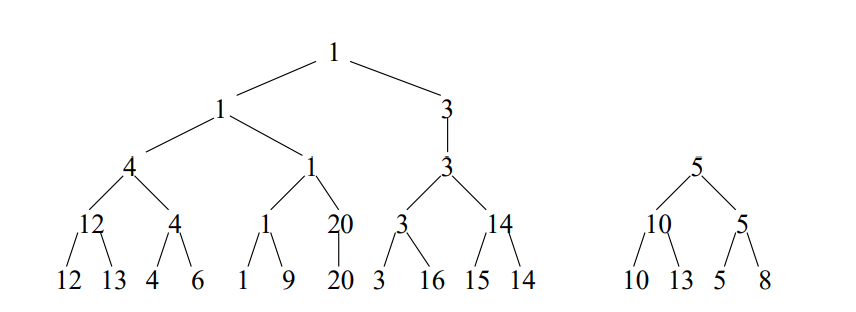
\includegraphics[width=18cm, height=6cm]{7.1.png}

Также хочу две оперцции:
\begin{enumerate}
    \item \textbf{link} --- берутся два дерева с одной высотой и объединяются (добавляется вершина, к которой ведут два корня, в нее записывается минимум из ее двух новых детей и ставится корень)
    \item \textbf{cut} --- возьму лист и буду подниматься вверх, пока не встречу число не равное числу на листе и отрежу получившееся поддерево. Очевидно, что все свойства нашего Quake Heap сохранятся и хуже не станет.
\end{enumerate}

\,

Пример выполнения cut: Беру третий лист в первом дереве и делаю cut по нему.

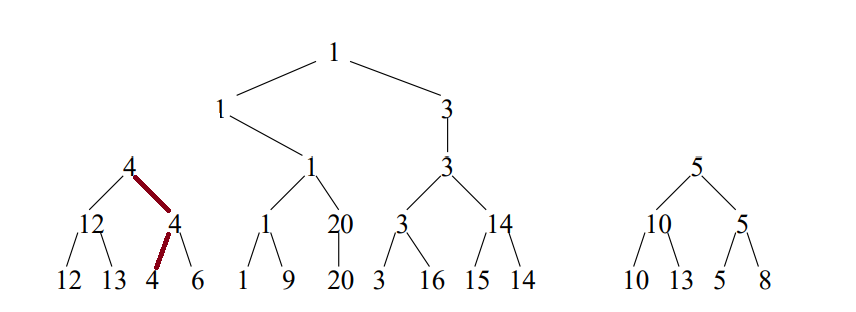
\includegraphics[width=18cm, height=6cm]{7.2.png}

И то, и то делается за O(1). 

Посмотрим тогда, как мы делаем наши операции.

\textbf{add(x)}:  создаем новое дерево. Работает за O(1)

\textbf{decrease\_key(v,y)}: делаем cut, меняем значение в листе(все будет работать за O(1), если в родителях хранить ссылку на лист, к которому они ссылаются).

\textbf{extract\_min()}: Найдем дерево с минимумом.(Бегаем по массивчику с корнями). Возьмем дерево и в наглую удалим путь нашего минимума:

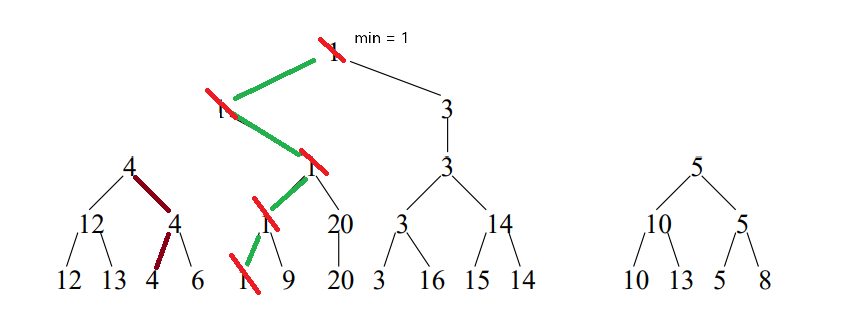
\includegraphics[width=18cm, height=6cm]{7.3.png}

Заметим, что так  у нас стало еще больше деревьев. Уменьшим их кол-во.

while есть два дерева одинаковой высоты, делаем их link (можем быстро так делать).

Пусть $n_i$ - кол-во вершин на i-ой высоте(поддерживается легко). Хочу поддерживать \textbf{инвариант} $n_{i+1}\leq \alpha n_i$, где $\alpha$ --- некоторая константа. $\alpha \in (\frac{1}{2},1)$. Получили, что высота O(log n).

Когда мы объединяли деревья, наш инвариант мог сломаться. Найдем min i, где условие сломалось, удалим все вершины с высотой >i.  Все починилось.


Хотим доказать, что extract\_min работает амортизированно за O(log n).

Пусть N - кол-во вершин, T - кол-во вершин, B - кол-во вершин с 1-им ребенком. $\phi = N+ T + \frac{B}{2\alpha-1}$. Докажем, что все работает

\begin{enumerate}
    \item[]  \textbf{add} --- N и T, увеличилось на 1. Амортизированно $O(1)$.
    \item[] \textbf{decrease\_key} --- увеличилось кол-во деревьев на 1, а еще кол-во вершин с 1 сыном увеличилось на 1.  Амортизированно $O(1)$.
    \item[] \textbf{extract\_min} --- по кускам оценим. Оценим истинное время и разность потенциалов всех операций до while. Настоящее время $T + log n + T-1$. Оценим $\phi$
    
    $\Delta n = -log n -log n$.
    
    $\Delta T =  +log n - T + log n$.
    
    $\Delta B = +log n$.

    Получаю $2log n$.  Дальнейшое док-во на некст лекции
\end{enumerate}

\pagebreak

\section{Продолжение куч.}
\subsection*{Cвязные списки.}

Хочу делать вот такие операции быстро:
\begin{enumerate}
    \item insert pos val
    \item erase  pos
    \item merge 
\end{enumerate}

\deff{Связный список} — структура данных состоящая из узлов, содержащих данные и ссылки на следующий и/или предыдущий узел списка.

Такую структуру данных удобно реализовывать на \deff{Pointer Machine} - модель хранения через указатели. 
\subsection*{Кучи.}
Вспомним двоичную:
\begin{enumerate}
    \item get\_min  O(1)
    \item extract\_min O(log n)
    \item add O(log n)
    \item decrease\_key O(log n)
    \item merge O(n+m)
\end{enumerate}
\deff{Биномиальная куча.}

Давайте начнем с чего-то более простого. \textbf{ Биномиальное дерево} $T_k$ --- дерево, определяемое для каждого k следующим образом: $T_0$ --- дерево, состоящее из одного узла; $T_k$ состоит из двух биномиальных деревьев $T_{k-
1}$, связанных вместе таким образом, что корень одного из них является дочерним узлом корня второго дерева. Дерево ранга k, обозначаем $T_k$.

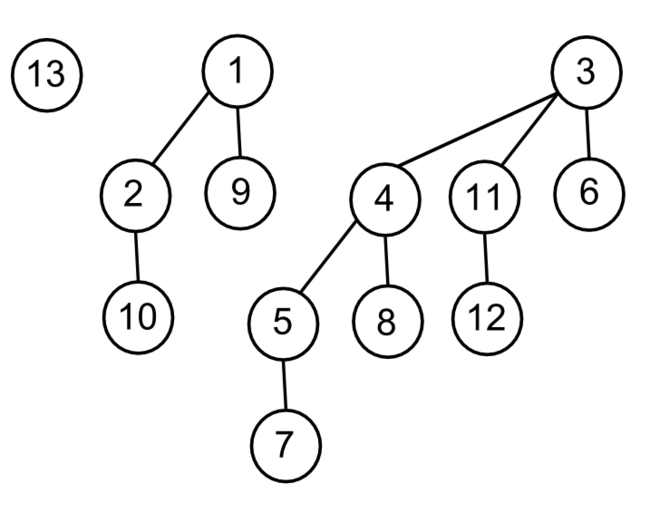
\includegraphics[width=8cm, height=6cm]{9.1.png}

Вот примеры деревья ранга 0, 2, 3, с записаннымм в вершины числами.

Давайте наложим на них свойства кучи и введем определение. 

\deff{Биноминальная куча} --- набор биноминальных деревьев(не больше одного дерева каждого ранга), дополненных свойством кучи. Заметим, что 3 дерева сверху - пример кучи. (Мы рассматиравем кучу на минимум).

Как храним?

Из родителя храним корень в самого левого сына. На каждом уровне в каждом дереве будем хранить двусвязный список (для всех отдельных деревьев - списки свои), а также положим корни в двусвязный список в порядке возрастания рангов деревьев.

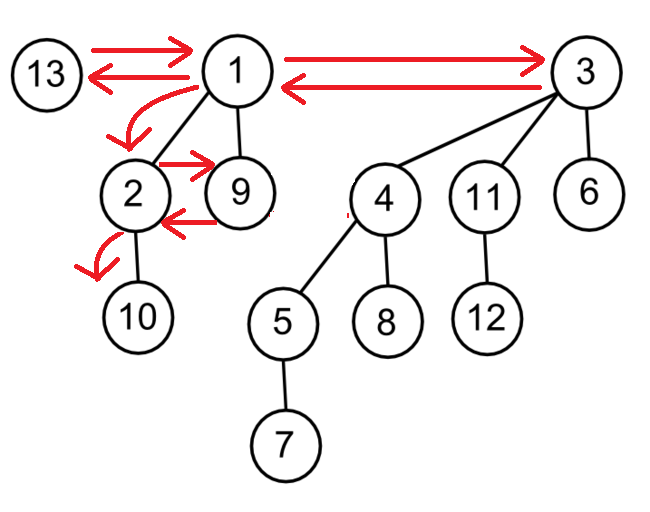
\includegraphics[width=8cm, height=6cm]{9.2.png}


Позамечаем всякие полезные свойства деревьев :

\textbf{\uline{Свойство 1}.}В дереве ранга k хранится $2^k$ вершин. Доказательство очевидно по индукции.

\textbf{\uline{Свойство 2}.} Высота $T_k$ равна k.  Доказательство очевидно по индукции.

\textbf{\uline{Свойство 3}.} У корня $T_k$ кол-во детей равно k. Доказательство очевидно по индукции.

\textbf{\uline{Свойство 4}.} Дети $T_k$ это  $T_0$,$T_1$, $T_2$,$\ldots$,$T_{k-1}$. Доказательство очевидно по индукции.

\textbf{\uline{Свойство 5}.} В $T_k$ на глубине d $C_k^d$ вершин. Шок! Доказательство очевидно по индукции!!!

Операции:

\begin{enumerate}
    \item \textbf{get\_min}  --- Поддерживаем ссылку на кучу с min (отдельный массив), при других операциях очевидно, как это поддерживать. O(1)

    \item \textbf{extract\_min} --- Минимум лежит в каком-то биноминальном дереве. Удалим вершину. Получим по св. 4 бин. деревья размера до k-1. Сделаем merge для искомой и получившийся удалением  вершины кучи. Работает за O(log n).
    
    \item \textbf{add}  --- Создадим кучу из добавляемого элемента и сделаем merge с нашей кучей. Работает за O(log n + log 1) = O(log n).
    
    \item \textbf{decrease\_key} --- Понижаем и делаем sift\_up, как в обычной куче. Работает за O(log n).

    \item \textbf{merge} --- бежим по списку корней первой кучи и второй. Посмотрим на ранги. Если $r_1\neq r_2$, то просто запишем меньшее. Если равны, то запишем смерженную (склеивать два дерева легко). До тех пор пока есть два дерева одинакового ранга, то смержим и добавим. Параллельно обновляем ссылку на минимум и т.п.. Работает за O(log(n) + log(m)). 
\end{enumerate}

\deff{\sout{Наркоманская} Фиббоначева куча.}

$T_0$ ---  1 вершина.

$T_k$ ---  k детей. Дадим каждому ребенку номер от 0 до k-1. Ранг дерева, начаниющегося в ребенке i $\geq $ i.

Деревья легкого поведения (очень много деревьев такого вида). $T_k^*$ --- дерево $T_k$, но без одного сына. Давайте у подвешешенных деревьем разрешим добавлять звездочки. $T_k^*$ --- в дальнейшем будет называться инвалидом.

\deff{Фиббоначева куча} --- набор таких деревьей, нам пофиг на ранги, просто набор, в вершинах деревьях храним числа, как  в обычной куче. ( В данном случае рассматривается куча на минимум)

\textbf{ФанФакт}. Ранг дерева размера n --- это O(log n).

$s_k$ --- min кол-во вершин в $T_k$. $s_0 =1$. $s_1 =2$.

$s_k = ?$ Давайте минимизируем кол-во вершин. Пусть i-ый ребенок будет ранга i, а также он будет инвалидом. Посчитаем кол-во вершин. 

$s_k = 1+ s_{k-2}+s_{k-3}+\ldots + s_0 = s_{k-1} +s_{k-2}$. (проверить это легко, раскройте $s_{k-1}$ по формуле и получаете изначальное). 

Получаем формулу такую же, как для чисел фиббоначи.

$F_n = \cfrac{\phi^n + \phi^{-n}}{\sqrt{5}}=O(\phi^n)$, где $\phi$ - коэф. золотого сечения.

Пусть $s_k \leq n < s_{k+1}$. $k\leq \log_{\phi} n<k+1$. Откуда и следует искомое.

Храним фиббоначеву так же, как и биноминальную. Поддерживаем ссылку на минимум, как в биноминальной куче.

Операции:

\begin{enumerate}
    \item \textbf{get\_min}  --- берем ссылку на минимальный. Работает за O(1)

    \item \textbf{extract\_min} ---  удалим вершину, дерево развалится и вставим их в список с корнями. Сделаем consolidate (сделаем каждого ранга не больше одного дерева).  Заведем массив длины log n. Пойду по двусвязному списку. Если я встречаю дерево ранга i и в нашем массиве по индексу i ничего не лежит, запишу ссылку на наше дерево в массив по индексу i. Если я встречаю дерево ранга i и в нашем массиве по индексу i что-то лежит, то я объединяю текущее дерево и то, которое лежит в массиве, и делаю дерево ранга i+1.(Это происходит просто добавлением сына в наше дерево, обновлением минимума и добавлением ссылок в двусвязные списки). Делаю так, пока повторений не будет. Сделаем эту кучу. 
    
    \item \textbf{add}  --- Создаем дерево ранга 0. Смержим. Победа. Работает за O(1).
    
    \item \textbf{decrease\_key} --- Если корень, то очев. Пусть не корень. Давайте обрежем дерево  и отправим вершину в конец кучи. Если та, у которой мы отобрали сына была со звездочкой, то такое нельзя терпеть (представьте, что у вас двух сыновей украли).Если она не корень(в случае корня просто понизим ранг и все супер), то давайте отрежем ее от вершины, к которой она привязана. Будем так подниматься наверх. Истинное время такой штуки это количество запусков. Амортизированное O(1).

    \item \textbf{merge} --- берем два списка с корнями, соединяем. Работает за O(1).
\end{enumerate}

Хотим амортизированно оценить. Пусть потенциал это кол-во деревьев + 2 на количество вершин со звездочкой. Заметим, что тогда extract\_min работает за log n. 


\pagebreak

\section{DSU или Union-Find Data Structure или СнМ.}

Даны $1,2,\ldots,n$. Запихнем их каждое в одно множество. Какие операции поддерживаем? Давайте назначим в каждом множестве представителя.

\begin{enumerate}
    \item \textbf{unite a b} --- объединить множество с элементом a и множество с элементов b в одно.
    \item \textbf{get a} --- вернуть представителя множества a.
\end{enumerate}

\textbf{Данный код не понадлежит копированию, мне еще контест засылать с ним.}

Реализация (тупая):
\begin{lstlisting}[mathescape]
vector<lli> prevv, sizee;
 
lli getleader(lli i) {
    if (prevv[i] == i) return i;
    return getleader(prevv[i]);
}
 
void union_items(lli a, lli b) {
    a = getleader(a);
    b = getleader(b);
 
    if (a != b) {
        prevv[a]=b;
    }
}
\end{lstlisting}

Давайте добавим оптимизаций. 

\deff{Эвристика объединения по рангу (ранговая)}. Давайте  подвешивать дерево с меньшим размером к дереву с большим. (иногда делают другие ранговые системы, например по самому глубокому листу, но нам это не особо нужно, используя эвристику сжатия пути)

В лекции рассматривается эвристика по самому глубокому листу, но это душно и не вкусно и бесполезно.

\deff{Эвристика сжатия пути}. Давайте при запросе getleader переподвешивать наши деревья за корень.

\begin{lstlisting}[mathescape]
vector<lli> prevv, sizee;
 
lli getleader(lli i) {
    if (prevv[i] == i) return i;
    prevv[i] = getleader(prevv[i]);
 
    return prevv[i];
}
 
void union_items(lli a, lli b) {
    a = getleader(a);
    b = getleader(b);
 
    if (a != b) {
        if (sizee[a] < sizee[b])
            swap(a, b);
 
        prevv[b] = a;
        sizee[a] += sizee[b];
    }
}
\end{lstlisting}
В main происходит примерно вот такое
\begin{lstlisting}[mathescape]
    prevv.resize(n);
    sizee.resize(n);
 
    for (lli i = 0; i < n; i++) {
        prevv[i] = i;
        sizee[i] = 1;
    }
\end{lstlisting}

Докажем за сколько это работает.

Введем последовательность $F(0)=1, F(n) = 2^{F(n-1)}$. степенная башня из n двоек.

$log_2^*n$ или Итерированный логарифм  --- минимальное k, что $F(k)\geq n$.

\textbf{Лемма.} Кол-во деревьев с рангом r не превосходит $\frac{n}{2^r}$. очевидно.

Введем g(v) - группа вершины v. $g(v) = log_2^*(r[v])$, где r[v] - ранг вершины v. Количество таких групп не больше чем итерированного логарифма от n.

\textbf{Лемма.} Кол-во вершин в группе g не превосходит $\frac{n}{F(g)}$. Очевидно.

Хочу доказать, что m вызовов get работют за $O(mlog_2^*n)$(при$m\geq n)$.

лекция 8 допилить доказательство
\pagebreak
\section{Хеширование.}

Хотим проверять строки  на равенство быстро. Сейчас мы умеем это делать за длину.

Допустим мы захотим все это делать быстрее чем за длину:
\begin{enumerate}
    \item add x
    \item remove x
    \item find x
\end{enumerate}

Нам поможет \uline{хеширование}! Хеш - функция, которая по объекту выдает число. Хотим, чтобы вызывая на разных получали разные числа, а на одинаковых получали одинаковое.

\uline{\textbf{Полиномиальный хеш.}}

Есть строка $s = s_0s_1\ldots s_{n-1}$, $s_i$ - символ.

Тогда $f(s) = \sum\limits_{i=0}^{n-1}s_i\cdot p^{n-i-1}$, где p - основание хеша. Но числа растут быстро и уже с длины 30 мы выйдем за  long long - плохо. Так что давайте брать все по модулю m, но из-за этого есть проблема. Строкам сопоставляются значения от 0 до m.

\uline{\textbf{Коллизия}} -  2 разных элемента дают один  хеш код.

Есть проблема в том, что зная код можно найти контртест. Поэтому давайте брать p - рандомное от 0 до m-1.

Оценим вероятность того, что хеши совпадут. Будем брать строки одинаковой длины (сравнивать разной в целом странно). Тогда их хеши:
\[f(s_1) = (\sum\limits_{i=0}^{n-1}s_1[i]\cdot p^{n-i-1}) \mod m;\,\,f(s_2) = (\sum\limits_{i=0}^{n-1}s_2[i]\cdot p^{n-i-1}) \mod m \]

Запишем разность и получим, что если хеши равны, то: 

\[0 =(\sum\limits_{i=0}^{n-1}(s_1[i]-s_2[i])\cdot p^{n-i-1}) \mod m\]

И получаем, что эти строки совпадут только тогда, когда p - корень вот такого многочлена:

\[g(x) =(\sum\limits_{i=0}^{n-1}(s_1[i]-s_2[i])\cdot x^{n-i-1}) \mod m\] 

Количество корней g(x) mod m не превосходит n-1 (теорема из математики, которое мы не будем доказывать).

$P(p$ - корень$) \leq \cfrac{n-1}{m}$,  а при больших m эта вероятность достаточно маленькая.

Хочется делать, чтобы $\gcd(p,m) = 1$, иначе могут использоваться в виде хешей не все числа от 0 до m, а это плохо.

Но и это не всегда спасает. Например, на Codeforces есть система взломов. То есть другой человек может посмотреть ваш код, посмотреть на ваши mod  и \sout{взломать вашу ж*пу} подобрать такие различные
строки, хеши которых совпадут. Поэтому рекомендуется генерировать случайные (достаточно большие) простые числа: 

\begin{lstlisting}[mathescape] 
 inline ll gen_random_prime(ll L = (int) 1e9) {
    L += rand() % 123456789;
    while (! is_prime(L)) ++L; $\text{// проверка на простоту за O(sqrt(n))}$
    return L;
 }
 \end{lstlisting}

Также хочется, чтобы $p>$ размера алфавита, иначе может быть коллизия. По факту мы пишем представление числа в p-ичной системе счисления, в случае если алфавит больше у нас начнется появляться коллизия еще на уровне представление в p-ичной системе счисления.

\textbf{Задача.} У нас есть сообщения молодых людей в России призывного возраста. Хотим понять встречается ли в них фамилия нашего президента. 

В тупую решается за O(nm). Хотим быстрее

Есть строка t. Давайте посчитаем для каждого префикса хеш:

$h[i] =(h[i-1]\cdot p +t_{i-1}) \mod m$.

Хотим посчитать  хеш подстроки $[l,r)$:

$h[r] = (t_0 \cdot p^{r-1} + t_1 \cdot p^{r-2} + \ldots t_{r-1}) \mod m$

$h[l] =(t_0 \cdot p^{l-1} + t_1 \cdot p^{l-2} + \ldots t_{l-1}) \mod m$

$h[l,r] = (h[r] - h[l]\cdot p^{r-l}) \mod m$.

Поставим промежуток размера m  с нуля и начнем его двигать вправо, проверяя хеши на совпадение с хешом нужной нам подстроки. Если совпало, то победили, иначе идем раньше.

\textbf{Как убрать еще коллизию?} Можно сделать двойное хеширование (n-ичное хеширование).

\textbf{Задача.} Дана строка s. Хочу посчитать количество различных подстрок. Давайте подсчитаем все возможные хеши  и победим. 

Очевидно, что может сломаться из-за одной коллизии. Давайте научимся считать такую вероятность:

\[p_c = 1 - \cfrac{m \cdot (m-1) \cdot \ldots \cdot (m-n+1)}{m^n}\]

Это вероятность того, то  n хешей совпадут. Тогда с помощью лютых мат. подсчетов (которых не было и не будет), при $n\geq \sqrt{2m}$, наша штука будет больше 0.5.

\textbf{Задача.} Пишем раунд на кф и хотим \uline{злостно взламывать} чужие решение на хеш коды (Находить 2 строки с одним хешом). Это легко делать: будем рандомить строки и добавлять хеши в какую-то мапу и исходя из прошлой задачи, можем понять, что это займет не оч много времени.

Иногда хочется хешировать не только строки. 

\uline{\textbf{Как хешируем множества чисел?}}

Пусть есть два множества $s_1 = \{\alpha_1,\ldots ,\alpha_n\}$, $s_2 = \{\beta_1,\ldots ,\beta_n\}$. 

Пусть $g(x) = rand()$, $x \in [0,m)$

$f(s_1) = g(\alpha_1) \xor g(\alpha_2) \xor \ldots g(\alpha_n)$.

Посчитаем теперь, колизию. Она будет $\frac{1}{2^b}$, где b - кол-во битов в рандоме.  

\textbf{Пример решения задачи:}

Задача - найти равные строки из данного множества.
\begin{lstlisting}[mathescape]
vector<string> s (n);
$\text{// ... считывание строк ...}$

$\text{// считаем все степени p, допустим, до 10000 - максимальной длины строк}$
const int p = 31;
vector<long long> p_pow (10000);
p_pow[0] = 1;
for (size_t i=1; i<p_pow.size(); ++i)
	p_pow[i] = (p_pow[i-1] * p)%mod+mod)%mod;

$\text{// считаем хэши от всех строк}$
$\text{// в массиве храним значение хэша и номер строки в массиве s}$
vector < pair<long long, int> > hashes (n);
for (int i=0; i<n; ++i)
{
	long long hash = 0;
	for (size_t j=0; j<s[i].length(); ++j)
		hash += ((s[i][j] - 'a' + 1) * p_pow[j]%mod+mod)%mod;
	hashes[i] = make_pair (hash, i);
}

$\text{// выводим ответ}$

\end{lstlisting}

\pagebreak

\section{Хеш-таблицы. Вероятности и всякое}

Пусть мы хотим реализовать set:
\begin{enumerate}
    \item add x
    \item remove x 
    \item find x
\end{enumerate}

Заведем массивчик, он будет состоять из m элементов. Дальше мы будем делать очень простую штуку

Как мы делаем операции?  Пусть есть Хеш функция $h: X \shortrightarrow \{0,1,2,\ldots,m-1\}$

\begin{enumerate}
    \item add x. Положим элемент в ячейку H(x).
    \item remove x - удалить из H(x)
    \item find x - зайти в элемент посмотреть null или не null.
\end{enumerate}

Что делать когда 2 раза в одну ячейку? Как бороться с коллизией

\deff{Способ 1. Метод цепочек.} 

В каждой ячейке храним связный список с элементами с таких хешом, записываем в тот связный списочек (храним уникальные элементы) удаляем и ищем столько же.  

Запросы работают за O(len) - может быть много, если цепочки большие.

Легко также сломать наш хеш.

Введем новое понятие:

\deff{Универсальная система хеш-функций.} Пусть H = $\{h_1,h_2,\ldots,h_k\}$.

Хочу:
$\forall a,b \in X: a\neq b:$ количество функций в $h_i \in H: h_i(a)=h_i(b)$ не превосходит $\cfrac{|H|}{m}$. Иная формулировка: вероятность коллизии у рандомно-выбранной $\leq \cfrac{1}{m}$.

Пусть такая есть (позже про это скажем). Давайте выберем одну из хеш-функций. Давайте оценим длина цепочки в среднем (C- цепочка):

$E(len)= E(\sum\limits_{x\in C} 1) = \sum\limits_{x\in C} E(1) = \sum p(x\in C) \leq \cfrac{n}{m}$. Берем $m = 2n$  и чиллим. Получим O(1).

Давайте покажем, что такие семейства существуют:

Пусть хотим хешировать числа $\{0,1,2,\ldots,t-1\}$, m - размер таблицы. Давайте выберем $p>t,p$ - простое. 

Пусть наше семейсто будет из всех функций такого вида:

$h(x) = ((a*x+b)\mod p)\mod m$; $0<a<p;0\leq b < p$

Возьмем какие-то x,y(не равные)

$h(x) = ((ax+b) \mod p) \mod m$

$h(y) = ((ay+b) \mod p) \mod m$

Заметим, что остатки по модулю p не равны (от противного очевидно). Тогда вероятность того, что хеши совпадут это максимум $\cfrac{1}{\frac{p}{m}}$. Тогда вся вероятность это $\cfrac{1}{\frac{p}{m}}\cdot \cfrac{p \cdot (\frac{p}{m}-1)}{p (p-1)} = \cfrac{1}{m}$  - \uline{доказали}, что такае есть

\deff{Способ 2. Открытая адресация.}

$m\geq n$. Добавления понятны. А допустим теперь случилась коллизия. Давайте вместо того, чтобы класть в текущую, будем класть в  ближайшую правую свободную (цикличную). 

Как удалить? аналогчино

\deff{Фильтр Блума}

\begin{enumerate}
    \item add x
    \item find x
\end{enumerate}

Псевдокод:
add:
\begin{lstlisting}[mathescape]
for i=1,...,k:
a[hi(x)]=true
\end{lstlisting}

find(x):
\begin{lstlisting}[mathescape]
for i=1,...,k:
  if(a[bi(x)] = false: return false;
return true;
\end{lstlisting}

Понятно как тут работает. Проблема, что find x может косячить. Работает как фильтр (пытаемся посмотреть равны ли, и если равны, то запустить более тяжеловесную функцию find)

\pagebreak

\section{Perfect Hashing}
%TODO: красивше

X - множество хешируемых элементов: $x_1,x_2,\ldots, x_n \in X$.

Хотим придумать $h: X \shortrightarrow \{0,1,2,\ldots,m-1\}$

$\forall i,j: h(x_i) \neq h(x_j)$.

$m = n^2$. Трачу $O(m)$  памяти:

H - семейство универсальных хеш-функий. Возьмем случайную хеш-функцию.(размера m). Возьмем случайную хеш-функцию. 

Оценим вероятность того, что есть коллизия:

$\forall x_i,x_j p(h(i)=h(x_j))\leq \cfrac{1}{m}$

p(есть коллизия) = 1 - p(нет колизии) = $1 - \cfrac{n^2-1}{n^2}^{\cfrac{n^2-n}{2}}$

E(кол-ва коллизий) = $\cfrac{n (n-1)}{2} \cdot \cfrac{1}{m}<\cfrac{1}{2}$

Окей. Как сделать по-другому.

Давайте за O(n) - доп памяти.  Возьмем какую-то хеш - фукнцию. Получу какие-то элементы у которых совпал кеш. Найду хеш-функцию для них  такую, что их хеши совпадать не будут. И теперь у меня двойная аутентификация --- у каждой штуки 2 хеш функции - 1 общая, другая - в группе. Тратим O(n) памяти и времени.

\pagebreak
\textbf{Идея графов.} m порядка n

$x_1,x_2,\ldots, x_n$. Возьму из семейства $h_1,h_2$ - случайные хеш-функции. Возьму $h_1(x_i) = u_i$, $h_2(x_i) = v_i$. Давайте я создам граф и соединю все $u_i,v_i$ - пары вершин ребром. Будет m вершин n m ребер. Если есть цикл - все заново. Вероятность, что есть цикл - маленькая. Получил, что мои компоненты - деревья. Для каждого ребра запишу x, которому он соответствует.

В каждую вершину буду записывать числа так, чтобы для каждого ребра  сумма была равна этому i (по модулю n). Это очевидно. Пример:

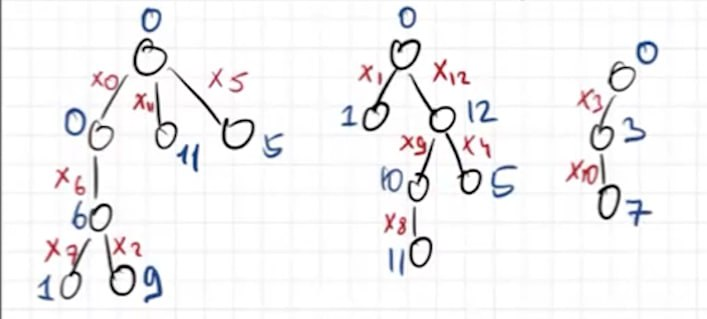
\includegraphics[width=12cm, height=5cm]{13.1.jpg}

Как теперь этим пользоваться? Вот у меня подается $h_1(x_i) = u, h_2(x_j)$. $h(x_i) = (a_u + a_v) \mod n $ - получили идеальный хеш для этих n чисел. 

\textbf{Хеши о деревьях.}

Пусть у нас есть всякие деревья. Назовем 2 Дерева \deff{изоморфными}, если существует такая перестановка, что для каждого ребра i,j из первого существует ребро между i,j во втором и обратно. Пример изоморфных:

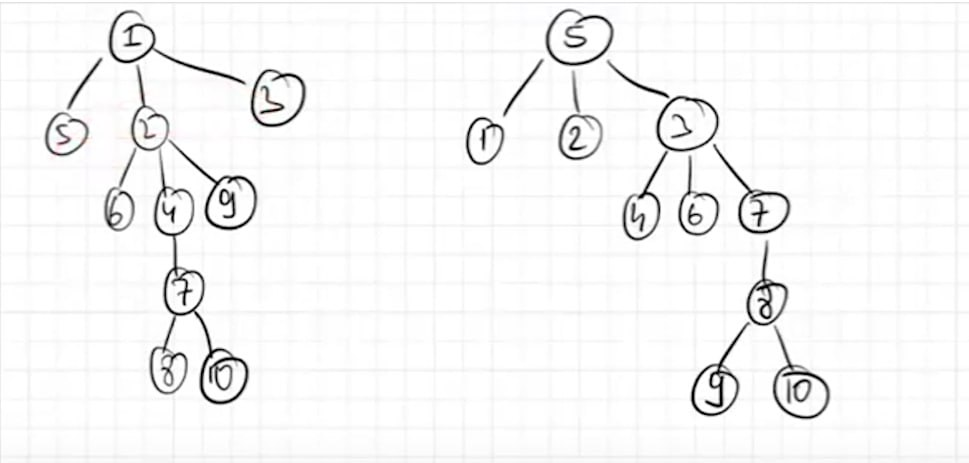
\includegraphics[width=12cm, height=6cm]{13.2.jpg}

Давайте считать \deff{хеши для  корневых деревьев}.

Давайте для каждой вершины я сопоставлю какое-то число, которое будет говорить о том, что у нас изоморфны деревья. То есть для каких-то двух вершин v и u:

$c_v = c_u \Leftrightarrow$ поддеревья и u,v - изоморфны.

Пусть есть вершина v и у нее есть дети. Пусть для них классы эквивалентности(те самые $c_v$) посчитаны. Пусть у всех листьев будут 0.  Возьму другую  вершину u. Эти деревья будут изоморфны, если  мультимножества, состоящие из классов эквивалентности детей, совпадут.

Давайте делать так: будем идти рекурсивно и для каждой вершины, если все классы эквивалентности (числа) детей этой вершины уже посчитанны, то:
Если в map нету мультимножество классов эквивалентности для текущей вершины, то добавлю и присвою ей новое число. Иначе достану число, которое надо присвоить из этой мапы.

Очевидно это работает!





\end{document}  
